\documentclass[a4paper]{jpconf}
\bibliographystyle{iopart-num}
\usepackage[binary-units=true]{siunitx}
\usepackage{listings}
\lstset{
  language=bash,
  captionpos=b,
  tabsize=8,
  frame=lines,
  numbers=left,
  numberstyle=\tiny,
  numbersep=5pt,
  breaklines=true,
  showstringspaces=false,
  basicstyle=\scriptsize\ttfamily\bfseries
}
%\usepackage[modulo]{lineno}
%\linenumbers
\usepackage{wrapfig}
\setlength{\abovecaptionskip}{-2pt}
\setlength{\belowcaptionskip}{-2pt}

\begin{document}

\title{System level traffic shaping in disk servers with heterogeneous protocols}

\author{Eric Cano and Daniele Francesco Kruse}

\address{European Organization for Nuclear Research CERN, CH-1211 Gen\`eve 23,
Switzerland}

\ead{eric.cano@cern.ch, daniele.francesco.kruse@cern.ch}

\begin{abstract}
Disk access and tape migrations compete for network bandwidth in CASTOR’s disk servers, over various protocols: RFIO, Xroot, root and GridFTP. As there are a limited number of tape drives, it is important to keep them busy all the time, at their nominal speed. With potentially 100s of user read streams per server, the bandwidth for the tape migrations has to be guaranteed to a controlled level, and not the fair share the system gives by default. Xroot provides a prioritization mechanism, but using it implies moving exclusively to the Xroot protocol, which is not possible in short to mid-term time frame,  as users are equally using all protocols. The greatest commonality of all those protocols is not  more than the usage of TCP/IP. We investigated the Linux kernel traffic shaper to control TCP/ IP bandwidth. The performance and limitations of the traffic shaper have been understood  in test environment, and satisfactory working point has been found for production.  Notably, TCP offload engines' negative impact on traffic shaping, and the limitations of  the length of the traffic shaping rules were discovered and measured. A suitable working  point has been found and the traffic shaping is now successfully deployed in the CASTOR  production systems at CERN. This system level approach could be transposed easily to other  environments.
\end{abstract}

\section{Introduction}
\subsection{CASTOR's disk staging and access patterns}
The CERN Advanced STORage manager (CASTOR) \cite{CASTORweb} is used to archive to tape the physics data of past and present physics experiments at CERN. The current size of the tape archive is more than \SI{91}{\peta\byte}. In 2012 alone, about \SI{30}{\peta\byte} of raw data were stored.

CASTOR organises data in files, which are stored in a disk staging area before migration to tape or after being recalled from tape. Each file is stored complete on one file system of one of the disk servers. The staging area is also used as a cache/work area where files are kept as long as possible. A garbage collector manages deletions. This double usage leads to a double access pattern, where the tape system competes with user access (interactive or batch processing) for accessing data in the disk servers.

A central scheduler, the stager, organises all data transfers to and from the staging areas. The tape system is scheduled with a ``freight train'' approach, where long lists of file transfers are sent to the tape servers for execution. The time delay between a scheduling decision and the actual transfer can be minutes. The precise location of the file on one disk server is pre-determined at scheduling time.

The stager limits the number of concurrent user accesses to disk servers with a slot system. But this does not guarantee efficient transfer from the user. Some experiment's frameworks open many files during the whole analysis session, where the actual data transfer for a given file is just a burst in the middle of a long, mostly idle session. This led operators to choose a high slot quota, and disk servers can end up with around 300 user connections. With all of those active, tape migrations can go as low as \SI[per-mode=symbol]{1}{\mega\byte\per\second}.

\subsection{Competition between end users and tape system for disk server bandwidth}

With the time delay between decision and actual transfer, the stager cannot guarantee an efficient data transfers for the tape server. Yet, an efficient tape transfer is fundamental as the tape drives are a scarce resource, shared by all users, and central for efficient migration to new tape media\cite{repack}. Disk pools are dedicated to a given experiment or task, so an inefficient access pattern has a controlled scope, however tape drives stuck waiting for data from disk servers have a global effect.

%\begin{figure}[h]
%\begin{center}
%\includegraphics{Data_transfer_schema}
%\end{center}
%\caption{\label{competition_for_disk}Competition for disk server bandwidth}
%\end{figure}


We therefore needed a mean to guarantee the bandwidth served to the tape drives and give them high priority. In addition, the disk servers contain a good number of disk spindles, but many of them are still connected to the network with a single \SI[per-mode=symbol]{1}{\giga\bit\per\second} interface: the network bandwidth is then the resource being competed for.

Today's tape drives typically achieve \SI[per-mode=symbol]{250}{\mega\byte\per\second}\cite{IBM} \cite{STK}. The tape servers buffer files in memory, and read/write up to 3 files in parallel, if they are small enough, so we need to guarantee between $\frac{\SI[per-mode=symbol]{250}{\mega\byte\per\second}}{3} = \SI[per-mode=symbol]{83}{\mega\byte\per\second}$ and \SI[per-mode=symbol]{250}{\mega\byte\per\second} from any disk server. This will not be achieved fully with a single \SI[per-mode=symbol]{1}{\giga\bit\per\second} interface, but with a fair share bandwidth as low as \SI[per-mode=symbol]{1}{\mega\byte\per\second}, we had a long way to go.

The CASTOR disk servers are accessed using several protocols: RFIO, XRoot, root and GridFTP. Tape servers use RFIO, but so do some user accesses. RFIO has no means to reserve bandwidth for a given user. On the other hand the tape servers are dedicated machines. The IP addresses are hence an appropriate criterion to discriminate between tape servers and other accesses.

\section{Traffic shaping as a mean to favour the tape servers}

As no application level means, neither central nor disk server level can guarantee the tape bandwidth, we investigated the system level. All the CASTOR infrastructure runs on Linux \cite{SLC}. The Linux kernel, beyond the classic IP chains,  contains many powerful network control features, allowing detailed routing and traffic control \cite{lartc}. The traffic control delays network packets on the output of an interface. As a consequence, this methodology only allows control for one direction out of two (migrations to tape, and not tape recalls), but securing the data to tape is the most important.

\subsection{Traffic control objectives}
We tried to guarantee 90\% of the bandwidth to the tape servers in case of mixed disk and tape traffic. We also want to still provide all of the bandwidth to any class of traffic in the absence of the other.

\subsection{Traffic control configuration}
By default the Linux kernel uses a``priority FIFO'' queuing discipline called (\verb#pfifo_fast#). This queuing discipline prioritises the IP packets based on the type of service (TOS) bits. In order to retain a behaviour as close as possible to the system defaults, we used the priority (\verb#prio#) queuing discipline, mimicking this default. The best effort TOS (which is where all the normal TCP traffic is) FIFO of this queuing discipline is in turn sent in a ``class base queuing" queuing discipline or \verb#cbq#. Our \verb#cbq# configuration contains 2 classes; one taking all traffic by default, and getting 10\% of the bandwidth (with possibility to borrow more from other idle classes). A second class gets the 90\% bandwidth. And finally a classifier assigns packets bound to tape servers to the second, high priority class. The classifier is a list of rules, which can select a single IP or a contiguous IP range.

In our case, there are no significant bidirectional data streams. So TCP packets carrying the ACK bit are usually small. Those packets are added to the high priority class in order to avoid penalizing incoming data transmission. Finally ssh protocol is also given high priority.

The detailed final configuration can be seen in appendix.

\subsection{Test environment}
The production environment does not provide a stable enough workload to provide reliable results. The workload was hence simulated with one machine identical to the production disk servers (with a single \SI[per-mode=symbol]{1}{\giga\bit\per\second} interface) and 2 client computers simulating respectively the tape and user clients, with a variable number of streams for each. The kernel used is Linux 2.6.18-274.17.1.el5, the test disk server had dual Intel Xeon E51500 @ 2.00GHz processor, with a Intel 80003ES2LAN Gigabit card (one link out of 2 was used).

The three machines were dedicated to the test, and the bandwidth was measured through the increase of the bytes transfer statistics in \verb#/proc/net/dev# over \SI{2}{\second}.

\section{Results}

\begin{figure}[h]
\begin{center}
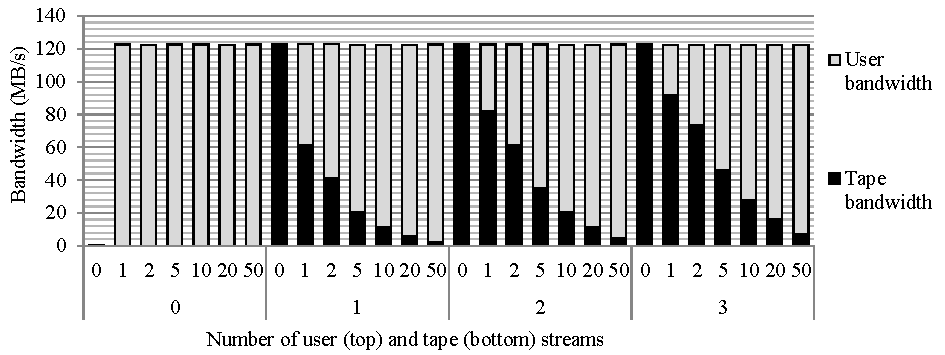
\includegraphics{Bandwidth_without_traffic_shaping}
\end{center}
\caption{\label{nots_bandwidth_plot}Default bandwidth distribution (stacked)}
\end{figure}

\begin{figure}[h]
\begin{center}
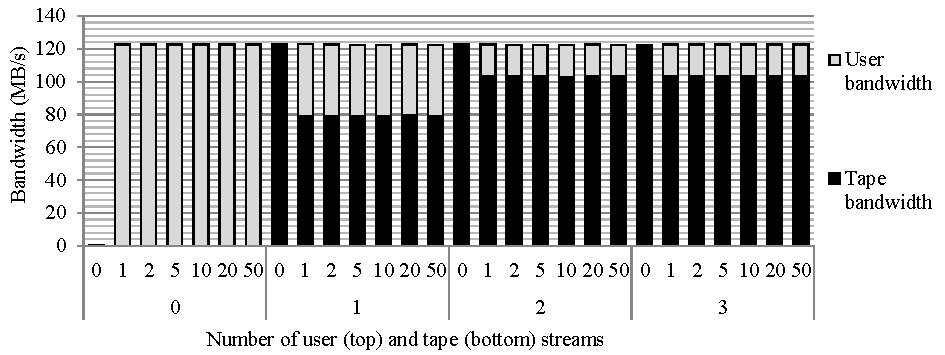
\includegraphics{Bandwidth_with_traffic_shaping}
\end{center}
\caption{\label{ts_bandwidth_plot}Traffic shaped bandwidth distribution (stacked)}
\end{figure}

During tests, various parameters and queuing disciplines were tested. Most notably, both borrowing and limitation to 90\% could not be achieved with other queuing disciplines. 

Additionally, the usage of TCP segmentation offload (TSO) engine with the traffic shaper led to unstable bandwidth, and a bandwidth ratio close to the non-traffic shaped one. Turning off the TSO costs more in processing time: the kernel and CPU see packets of network MTU (standard Ethernet MTU of \SI{1500}{\byte} in our case), and has to process and filter proportionality more packets. With the TSO on, a network capture showed packets of \SI{64}{\kilo\byte}.

The bandwidth ratio for various numbers of tape and user streams, for default set-up (where we get the expected fair share distribution), and with traffic control (TSO off) are shown in figures \ref{nots_bandwidth_plot} and \ref{ts_bandwidth_plot}. The values are the averages over several runs of the test.

The result is not exactly the expected 90\% ratio: with only one tape stream, we only reach a ratio of $\approx65\%$, and with at least two, the ratio becomes a stable $\approx84\%$.

\begin{wrapfigure}{L}{0.5\textwidth}
\begin{center}
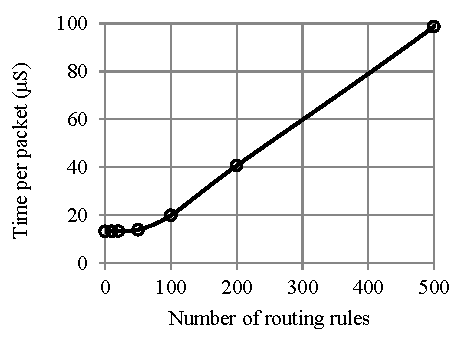
\includegraphics{Time_per_packet}
%%\hspace{2pc}%
%%\begin{minipage}[b]{14pc}
\caption{\label{time_per_packet}Time per packet against number of classification rules}
%%\end{minipage}
\end{center}
\end{wrapfigure}

The number of hosts listed in the tape host list also had an impact on performance, especially with a raised packet rate in the absence of TSO. We artificially increased the number of IP prioritization rules up to 2000 to measure their costs and assess the practical limits for the number of IP addresses. The average time per packet was deduced from the bandwidth measurements (making the assumption that the majority of packets were a full \SI{1500}{\byte}). This measurement is shown on figure \ref{time_per_packet}.

The measurements show an initial plateau where the time to process the classification rules is hidden by the time to send the packet over the wire ($\frac{\SI{1500}{\byte}}{\SI[per-mode=symbol]{1}{\giga\bit\per\second}}=\SI{12}{\micro\second}$). We then have a clean linear progression. The slope yields a processing time per rule of $\approx\SI{200}{\nano\second}$. This gives a budget of about 60 rules, not taking into account other processing overhead for packet processing. The measurements show that the limit is in our case closer to 50 rules at most.

With faster interfaces, the affordable number of rules decreases linearly, to the point of becoming impractical (about 5 only) for a $\SI[per-mode=symbol]{10}{\giga\bit\per\second}$.

\section{Deployment to production}
At CERN, we had 122 tape servers at deployment time, 11 network range based rules were enough to discriminate tape traffic. The traffic control script as show in appendix has been turned into a system service and deployed on live systems. The traffic control rules can be turned on an off at any moment without disrupting the network data flow.

Long term logs of the tape activity showed that before applying the traffic shaping, many days saw a significant fraction ($10-30\%$, sometimes more) of the data volume transferred to tape at less than $10\%$ of the maximum speed. This fraction dropped to $0.5\%$ on the worst days after applying the traffic shaping. No degradation of performance from the user's perspective was documented.

\section{Conclusions}
During a crunch in operations, the Linux kernel's powerful network control features proved invaluable to work around system overload. Some features had to be understood in a test environment, due to imprecise documentation, but the expected result was met.

This solution remains short term and only covers migrations to tape, but not recalls from tape. For the longer term, we are currently looking into additional tape staging area, allowing fully controlled scheduling, and distributed storage like a reliable array of inexpensive nodes (RAIN) like Ceph, where traffic would be evened out over many nodes, eliminating hotspots \cite{Ceph}.

\appendix
\section*{Appendix: the configuration script}
\begin{lstlisting}[caption={Traffic control setting script},label=tshape_script]
# Turn off TCP segmentation offload: kernel sees the details 
# of the packets routing
/sbin/ethtool -K eth0 tso off

# Flush the existing rules (gives an error when there are none)
tc qdisc del dev eth0 root 2> /dev/null

# Duplication of the default kernel behavior
tc qdisc add dev eth0 parent root handle 10: prio bands 3\
        priomap 1 2 2 2 1 2 0 0 1 1 1 1 1 1 1 1
		
# Creation of the class based queuing
tc qdisc add dev eth0 parent 10:1  handle 101: cbq bandwidth 1gbit avpkt 1500
tc class add dev eth0 parent 101: classid 101:10 cbq weight 90 split 101:\
        defmap 0 bandwidth 1gbit \
        prio 1 rate 900mbit maxburst 20 minburst 10 avpkt 1500
tc class add dev eth0 parent 101: classid 101:20 cbq weight 10 split 101:\
        defmap ff bandwidth 1gbit\
        prio 1 rate 100mbit maxburst 20 minburst 10 avpkt 1500
        
# Prioritize ACK packets
tc filter add dev eth0 parent 101: protocol ip prio 10 u32\
        match ip protocol 6 0xff\
        match u8 0x05 0x0f at 0\
        match u16 0x0000 0xffc0 at 2\
        match u8 0x10 0xff at 33\
        flowid 101:10
        
# Prioritize SSH packets
tc filter add dev eth0 parent 101: protocol ip prio 10 u32\
        match ip sport 22 0xffff flowid 101:10

# Prioritize network ranges of tape servers
tc filter add dev eth0 parent 101: protocol ip prio 10 u32 match ip\
        dst <Network1>/<bits1> flowid 101:10
tc filter add dev eth0 parent 101: protocol ip prio 10 u32 match ip\
        dst <Network2>/<bits2> flowid 101:10
# <etc..>
\end{lstlisting}


\section*{References}
\begin{thebibliography}{6}
\bibitem{CASTORweb}CASTOR homepage {\it{}http://cern.ch/castor}
\bibitem{repack}Kruse D F 2013 {\it{}The Repack Challenge} Unpublished paper presented at CHEP 2013, Amsterdam 
\bibitem{IBM}IBM enterprise tape drives {\it{}http://ibm.com/systems/storage/tape/drives/}
\bibitem{STK}Oracle StorageTek T10000C Tape Drive {\it{}http://www.oracle.com/us/products/servers-storage/storage/tape-storage/t10000c-tape-drive/overview/index.html}
\bibitem{SLC}Scientific Linux CERN {\it{}http://cern.ch/linux/scientific.shtml}
\bibitem{lartc}Linux advanced routing and traffic control {\it{}http://www.lartc.org/lartc.pdf}
\bibitem{Ceph}Weil S. A. 2007 Ceph: Reliable, scalable, and high-performance distributed storage {\it{}http://ceph.com/papers/weil-thesis.pdf}
\end{thebibliography}
\end{document}
